% paper/sections/13d_density_ratio.tex
%
% V6: 密度比 sweep convergence (rho_r in {2,10,100,833}, N in {24,32})
% V7: IMEX-BDF2 二相時間精度 (Linf err vs dt)
% ═══════════════════════════════════════════════════════════════════════════════
\subsection{密度比収束と IMEX-BDF2 時間精度}
\label{sec:varrho_dc_convergence}

\subsubsection{\texorpdfstring{V6：密度比掃引 ($\rho_r = 2 \to 833$)}{V6：密度比 sweep (rho_r = 2 to 833)}}
\label{sec:density_ratio_sweep}
\label{sec:interface_crossing}

\paragraph{検証対象．}
分相 PPE + DC + HFE 統合（\autoref{sec:split_ppe_motivation}〜\autoref{sec:U6_split_ppe_dc_hfe}）に対応する，
圧力ジャンプ・毛管射影結合系の FCCD 界面輸送 / UCCD6 対流 /
Hermite Field Extension (HFE) による片側延長・曲率データ供給 / 圧力ジャンプ表面張力 /
分相 FCCD PPE + 欠陥補正 + 射影後面速度閉包 /
毛管成分の圧力勾配射影 / アフィン圧力履歴面加速度の構成が，
密度比 $\rho_r = \rho_l/\rho_g \in [2, 833]$（最大は水--空気の $\sim 833$；高密度比 LS の系統解析は~\cite{SussmanSmereka1997,Tryggvason2011}）で
\textbf{ブローアップしない}ことを確認する．
本検証は，一括 smoothed-Heaviside 解法で顕在化しうる密度ジャンプ越え問題に対する
分相・ジャンプ分解経路の応答評価でもある．
圧力ジャンプ形式では Laplace 跳び $\sigma/r$ は PPE の界面結合に埋め込まれるため，
出力される $p$ は絶対圧ではなく射影補正圧である．したがって本 V6 では
$u_\infty^{\mathrm{end}}$，CLS 体積ドリフト，および
$|\Delta p_{\mathrm{corr}}|/(\sigma/r)$ をソルバ診断として測る．

\paragraph{設定．}
半径 $r=0.25$ の静止液滴，$\rho_l=\rho_r$, $\rho_g=1$, $\sigma=1$．
$\rho_r \in \{2,10,100,833\}$, $N \in \{24,32\}$．
各ケース $8$ step，CFL multiplier $0.50$．
検証経路は上記の圧力ジャンプ・毛管射影結合系に固定し，通常 CCD/FVM-PPE 経路とは分離する．

\paragraph{結果．}
\begin{table}[!ht]
\caption{V6：圧力ジャンプ・毛管射影結合系による密度比掃引}
\label{tab:V6_density_ratio}
\PaperCaptionNote{全 8 ケースでブローアップなし． $|\Delta V_\psi|/V_{\psi,0}$ は全ケースで round-off floor（$\le 1.2\times10^{-16}$）に留まり，毛管成分の圧力勾配射影後の $u_\infty^{\mathrm{end}}$ は最大でも $1.3\times10^{-9}$ である． $|\Delta p_{\mathrm{corr}}|/(\sigma/r)$ は pressure-jump PPE の補正圧診断であり， Laplace 絶対圧誤差ではない．}
\centering\small
\begin{tabular}{r r r r r}
\toprule
$\rho_r$ & $N$ & $u_\infty^{\mathrm{end}}$ & $|\Delta V_\psi|/V_{\psi,0}$ & $|\Delta p_{\mathrm{corr}}|/(\sigma/r)$ \\
\midrule
2    & 24 & $1.020\times 10^{-12}$ & $1.183\times 10^{-16}$ & $0.750$ \\
2    & 32 & $0.000$ & $0.000$ & $1.003$ \\
\midrule
10   & 24 & $1.238\times 10^{-9}$ & $1.183\times 10^{-16}$ & $0.739$ \\
10   & 32 & $0.000$ & $0.000$ & $1.003$ \\
\midrule
100  & 24 & $3.927\times 10^{-10}$ & $1.183\times 10^{-16}$ & $0.737$ \\
100  & 32 & $0.000$ & $0.000$ & $1.002$ \\
\midrule
833  & 24 & $3.371\times 10^{-10}$ & $1.183\times 10^{-16}$ & $0.758$ \\
833  & 32 & $0.000$ & $0.000$ & $1.002$ \\
\bottomrule
\end{tabular}
\end{table}

\begin{figure}[!ht]
\centering
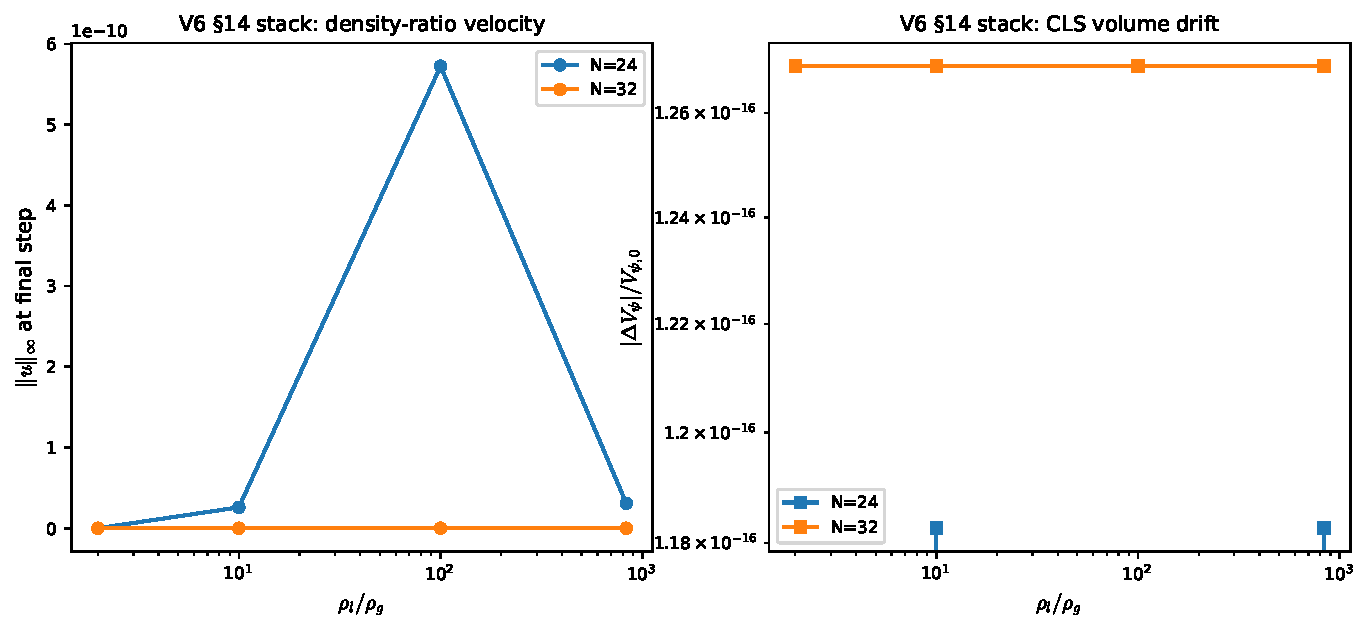
\includegraphics[width=0.92\linewidth]{figures/ch13_v6_density_ratio.pdf}
\caption{V6：密度比収束掃引}
\label{fig:V6_density_ratio}
\PaperCaptionNote{$u_\infty^{\mathrm{end}}$（左）は毛管成分の圧力勾配射影後に全密度比で $O(10^{-9})$ へ落ちる．右は CLS 体積 drift であり， 全ケース round-off floor に留まる．}
\end{figure}

\begin{figure}[!ht]
\centering
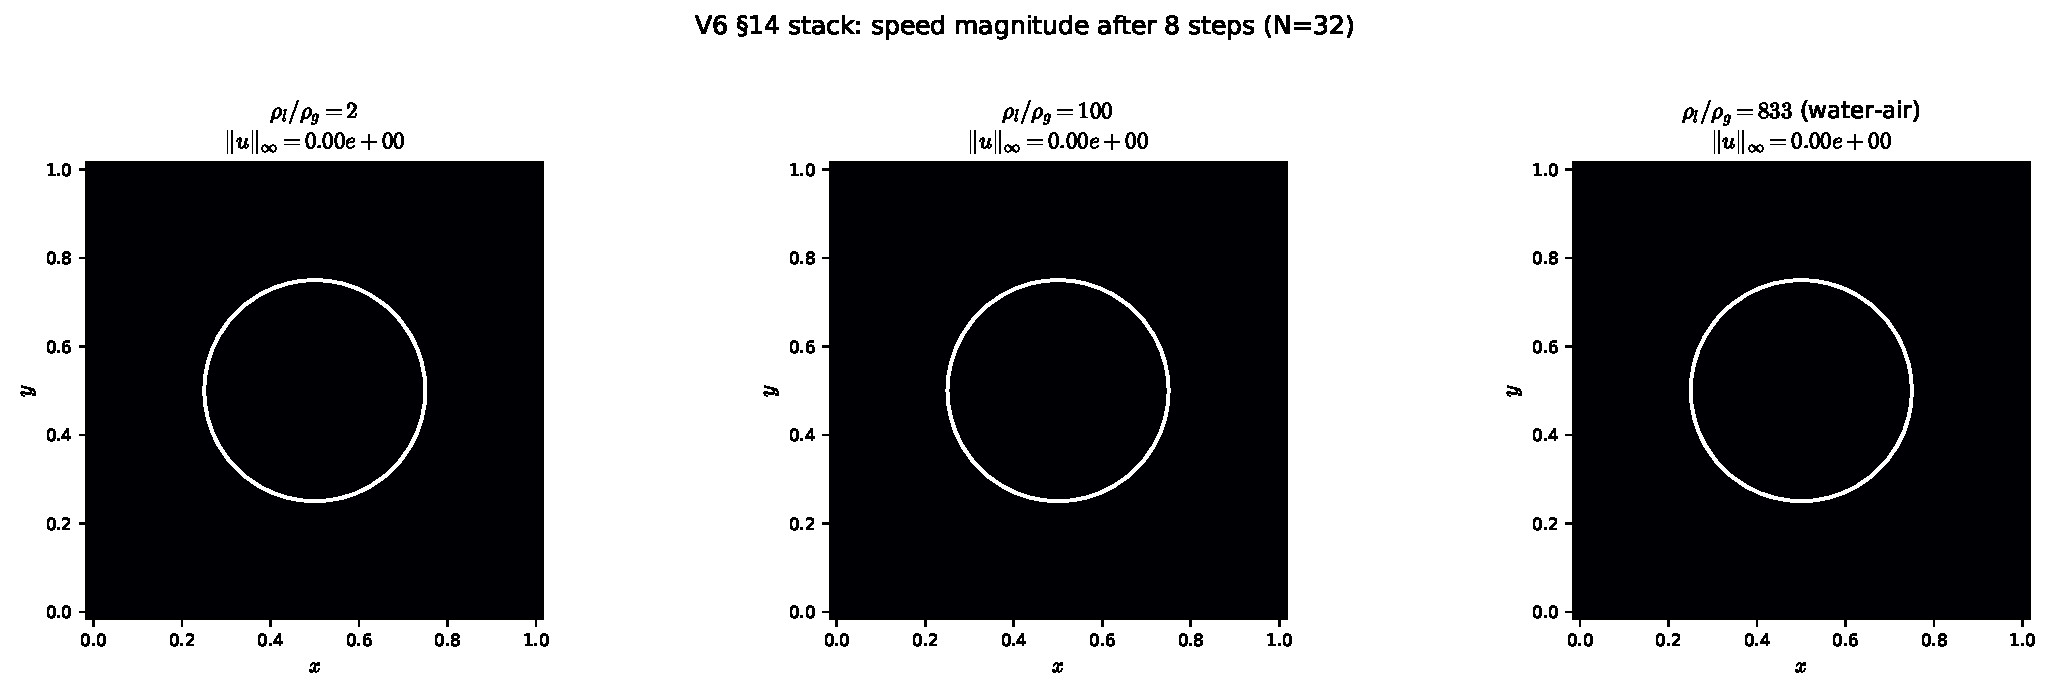
\includegraphics[width=0.98\linewidth]{figures/ch13_v6_density_ratio_fields.pdf}
\caption{V6：密度比掃引の終端速度場}
\label{fig:V6_density_ratio_fields}
\PaperCaptionNote{$\rho_l/\rho_g \in \{2, 100, 833\}$，$N=32$，圧力ジャンプ・毛管射影結合系（FCCD, UCCD6, HFE, 圧力ジャンプ付き分相 PPE/DC, 毛管成分の圧力勾配射影, 射影後面速度閉包, アフィン圧力履歴面加速度）．白円は界面 $\psi = 0.5$．各パネルで個別 $v_{\max}$ を取り，毛管成分の圧力勾配射影後の面バランスが密度比に依存せず丸め誤差近傍の速度場を与えることを確認する．}
\end{figure}

\paragraph{判定と制約条件．}
\begin{itemize}\setlength{\itemsep}{0pt}
  \item \textbf{主指標（合格条件）}：(a) 全 $8$ ケースで\textbf{ブローアップなし}
        （水--空気相当 $\rho_r=833$ を含む）\checkmark，
        (b) $|\Delta V_\psi|/V_{\psi,0} \le 1.2\times10^{-16}$ で CLS 体積は実質保存\checkmark，
        (c) $u_\infty^{\mathrm{end}}\le 1.3\times10^{-9}$ で毛管面バランスが丸め誤差近傍に閉じる\checkmark．
  \item \textbf{補助指標（scale 確認）}：
        $|\Delta p_{\mathrm{corr}}|/(\sigma/r) \sim 0.74$--$1.01$ は
        pressure-jump PPE の補正圧 diagnostic（§\ref{sec:verification}「圧力出力の取り扱い」参照；
        Laplace 絶対圧誤差ではない）であり，合格基準には含めない．
  \item 本 V6 は通常 CCD/FVM-PPE ではなく
        FCCD, UCCD6, HFE, 圧力ジャンプ付き分相 PPE/DC,
        毛管成分の圧力勾配射影，射影後面速度閉包，アフィン圧力履歴面加速度の経路を直接検証する．
\end{itemize}
検証対応：式~\eqref{eq:split_ppe}，\autoref{sec:split_ppe_motivation} の分相 PPE，
\autoref{sec:verify_split_ppe_dc}（DC），\autoref{sec:U6_split_ppe_dc_hfe}（HFE）に対し，
密度比掃引の終端速度，CLS 体積ドリフト，補正圧スケールを測定する．

\FloatBarrier

\subsubsection{V7：IMEX-BDF2 二相時間精度}
\label{sec:imex_bdf2_twophase_time}

\paragraph{検証対象．}
密度比 $\rho_r > 1$ の二相 NS において，IMEX-BDF2 時間離散~\cite{AscherRuuthSpiteri1997,HairerWanner1996}
（\autoref{ch:time_integration}）を含む圧力ジャンプ・毛管射影結合系の
FCCD 界面輸送 + TVD-RK3，UCCD6 対流 + IMEX-BDF2，
HFE 曲率，Ridge--Eikonal 再初期化，圧力ジャンプ型分相
FCCD PPE + 欠陥補正，毛管成分の圧力勾配射影，射影後面速度閉包，アフィン圧力履歴面加速度
を同時に使ったときの実効時間精度を，
参照解との差で評価する．これは BDF2 単体の次数検証ではなく，
界面輸送・再初期化・圧力ジャンプ PPE を含む結合系診断である．

\paragraph{設定．}
$\rho_l=10,\rho_g=1$ ($\rho_r=10$), 液滴半径 $r=0.25$, $\sigma=1$．
$N=24$, $T=0.02$．初期速度は液相内に
$u_0=0.02\cos(2\pi y)H_\varepsilon$, $v_0=-0.02\cos(2\pi x)H_\varepsilon$ を与える．
$n_{\mathrm{step}}\in\{8,16,32\}$ を粗解，$n_{\mathrm{ref}}=64$ を参照解とし，
Ridge--Eikonal 再初期化は全 step で有効化する．

\paragraph{結果．}
\begin{table}[!ht]
\caption{V7：圧力ジャンプ・毛管射影結合系の二相時間精度診断}
\label{tab:V7_imex_bdf2_time}
\PaperCaptionNote{参照は $n_{\mathrm{ref}}=64$．毛管成分の圧力勾配射影を含む圧力ジャンプ・毛管射影結合系での最終半減の観測収束率は $\mathbf{1.59}$ となる．純粋な 2 次には未達だが，分離診断は BDF2 係数ではなく圧力ジャンプを含む結合系が支配因子であることを示す．連続比は誤差 $\|e\|_\infty$ の直前行に対する比（$e^{(i-1)} / e^{(i)}$）であり，全半減が $\Delta t$ 比 $= 2$ のため収束率 $= \log_2(\text{連続比})$．}
\centering\small
\begin{tabular}{r r r r}
\toprule
$n_{\mathrm{step}}$ & $\Delta t$ & $\|e\|_\infty$ & 連続比 \\
\midrule
8    & $2.50\times 10^{-3}$ & $2.498\times 10^{-6}$ & ---  \\
16   & $1.25\times 10^{-3}$ & $1.068\times 10^{-6}$ & $2.34$ \\
32   & $6.25\times 10^{-4}$ & $3.546\times 10^{-7}$ & $3.01$ \\
\midrule
\multicolumn{3}{r}{細格子側局所収束率} & $\mathbf{1.59}$ \\
\bottomrule
\end{tabular}
\end{table}

\begin{figure}[!ht]
\centering
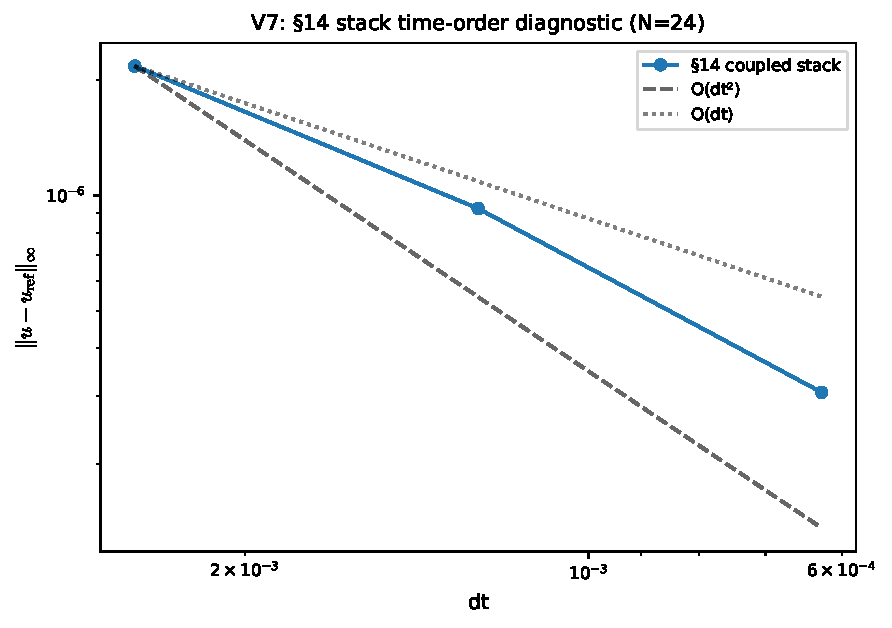
\includegraphics[width=0.92\linewidth]{figures/ch13_v7_imex_bdf2_time.pdf}
\caption{V7：IMEX-BDF2 二相時間精度}
\label{fig:V7_imex_bdf2_time}
\PaperCaptionNote{圧力ジャンプ・毛管射影結合系全体での参照解差を log-log 表示する．毛管成分の圧力勾配射影後の最終半減では収束率 $1.59$ となり，毛管圧力ジャンプ / アフィン FCCD 射影の界面帯誤差が実効次数を支配する．}
\end{figure}

\paragraph{判定と制約条件．}
\begin{itemize}\setlength{\itemsep}{0pt}
  \item 観測された最終局所収束率は $\mathbf{1.59}$．BDF2 単体の $2.00$ には届かないが，
        毛管結合系の実効次数として $1.5$ 近傍に位置する．
  \item \textbf{分離診断（毛管圧力ジャンプ/射影の界面帯律速）}：
        参照解品質，再初期化間隔，界面輸送，表面張力，二相係数を分離した補助診断では，
        $n_{\mathrm{ref}}=128$ でも収束率は $1.59$ 近傍に留まり，
        界面輸送を止めても同程度の実効次数が残る．一方，$\sigma=0$ では velocity error が
        数桁低下し，最大誤差は $\psi\simeq0.5$ の界面帯に局在する．
        したがって支配因子は BDF2 係数や reinitialization cadence ではなく，
        毛管圧力ジャンプ / アフィン FCCD 射影の界面帯誤差である
        （対照実験表は付録~\ref{app:v7_imex_bdf2_rca}）．
  \item \textbf{Type-D 合格 ($\triangle$, 毛管結合系律速)} —
        本稿では V7 を「BDF2 単体の純粋次数」ではなく「圧力ジャンプを含む毛管結合系下の
        実効次数」として測定する diagnostic とする．
        観測収束率 $1.59$ は，圧力ジャンプを含む界面帯低正則性を含む縮約下では
        \emph{毛管結合系に律速}されており，毛管ジャンプ/射影の
        時間離散を構造的に上げない限り $2.0$ への合格化は理論上望めない．
        これは Type-D（理論的下限; §\ref{sec:verification} の
        Type 分類および表~\ref{tab:V_verdict_types} 参照）として記録する．
        BDF2 単体の設計次数 $2$ は U8（§12）で既に独立検証済み．
\end{itemize}
検証対応：\autoref{ch:time_integration} の IMEX-BDF2 と
\autoref{sec:eikonal_reinit} の再初期化，\autoref{sec:split_ppe_motivation} の
圧力ジャンプ PPE と毛管成分の圧力勾配射影に対し，二相結合系の実効収束率を測定する．

\FloatBarrier
